
So far, we have learned about several IR units such as modules, functions, basic blocks, and instructions. We have also learned about some logical units such as CFG and call graphs. In this section, we are going to look at a more logical IR unit: a loop.

Loops are ubiquitous constructions that are heavily used by programmers. Not to mention that nearly every programming language contains this concept, too. A loop repeatedly executes a certain number of instructions multiple times, which, of course, saves programmers lots of effort from repeating that code by themselves. However, if the loop contains any inefficient code – for example, a time-consuming memory load that always delivers the same value – the performance slowdown will also be magnified by the number of iterations.

Therefore, it is the compiler's job to eliminate as many flaws as possible from a loop. In addition to removing suboptimal code from loops, since loops are on the critical path of the runtime's performance, people have always been trying to further optimize them with special hardware-based accelerations; for example, replacing a loop with vector instructions, which can process multiple scalar values in just a few cycles. In short, loop optimization is the key to generating faster, more efficient programs. This is especially important in the high-performance and scientific computing communities. 

In this section, we are going to learn how to process loops with LLVM. We will try to tackle this topic in two parts:

\begin{itemize}
\item Learning about loop representation in LLVM
\item Learning about loop infrastructure in LLVM
\end{itemize}

In LLVM, loops are slightly more complicated than other (logical) IR units. Therefore, we will learn about the high-level concept of a loop in LLVM and its terminologies first. Then, in the second part, we are going to get our hands on the infrastructure and tools that are used for processing loops in LLVM.

Let's start with the first part.

\subsubsubsection{10.4.1\hspace{0.2cm}Learning about loop representation in LLVM}

A loop is represented by the Loop class in LLVM. This class captures any control flow structure that has a back edge from an enclosing basic block in one of its predecessor blocks. Before we dive into its details, let's learn how to retrieve a Loop instance.

As we mentioned previously, a loop is a logical IR unit in LLVM IR. Namely, it is derived (or calculated) from physical IR units. In this case, we need to retrieve the calculated Loop instances from AnalysisManager – which was first introduced in Chapter 9, Working with PassManager and AnalysisManager. Here is an example showing how to retrieve it in a Pass function:

\begin{lstlisting}[style=styleCXX]
#include "llvm/Analysis/LoopInfo.h"
…
PreservedAnalyses run(Function &F, FunctionAnalysisManager
&FAM) {
	LoopInfo &LI = FAM.getResult<LoopAnalysis>(F);
	// `LI` contains ALL `Loop` instances in `F`
	for (Loop *LP : LI) {
		// Working with one of the loops, `LP`
	}
…
}
\end{lstlisting}

LoopAnalysis is an LLVM analysis class that provides us with a LoopInfo instance, which includes all the Loop instances in a Function. We can iterate through a LoopInfo instance to get an individual Loop instance, as shown in the preceding code.

Now, let's look into a Loop instance.

\hspace*{\fill} \\ %插入空行
\noindent
\textbf{Learning about loop terminologies}

A Loop instance contains multiple BasicBlock instances for a particular loop. LLVM assigns a special meaning/name to some of these blocks, as well as the (control flow) edges among them. The following diagram shows this terminology:

\hspace*{\fill} \\ %插入空行
\begin{center}
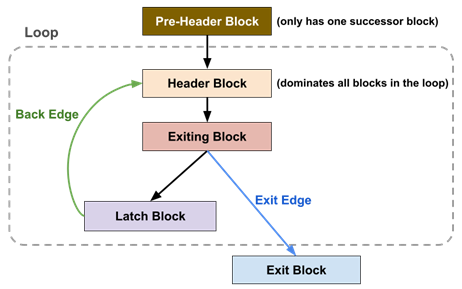
\includegraphics[width=0.9\textwidth]{content/3/chapter10/images/8.png}\\
Figure 10.8 – Structure and terminology used in a loop
\end{center}

Here, every rectangle is a BasicBlock instance. However, only blocks residing within the dash line area are included in a Loop instance. The preceding diagram also shows two important control flow edges. Let's explain each of these terminologies in detail:

\begin{itemize}
\item Header Block: This block marks the entry to a loop. Formally speaking, it dominates all the blocks in the loop. It is also the destination of any back edge.

Pre-Header Block: Though it is not part of a Loop, it represents the block that has the header block as the only successor. In other words, it's the only predecessor of the header block.

The existence of a pre-header block makes it easier to write some of the loop transformations. For instance, when we want to hoist an instruction to the outside of the loop so that it is only executed once before entering the loop, the pre-header block can be a good place to put this. If we don't have a pre-header block, we need to duplicate this instruction for every predecessor of the header block.

\item Back Edge: This is the control flow edge that goes from one of the blocks in the loop to the header block. A loop might contain several back edges.

\item Latch Block: This is the block that sits at the source of a back edge.

\item Exiting Block and Exit Block: These two names are slightly confusing: the exiting block is the block that has a control flow edge – the Exit Edge – that goes outside the loop. The other end of the exit edge, which is not part of the loop, is the exit block. A loop can contain multiple exit blocks (and exiting blocks).
\end{itemize}

These are the important terminologies for blocks in a Loop instance. In addition to the control flow structure, compiler engineers are also interested in a special value that might exist in a loop: the induction variable. For example, in the following snippet, the i variable is the induction variable:

\begin{lstlisting}[style=styleCXX]
for (int i = 0; i < 87; ++i){…}
\end{lstlisting}

A loop might not contain an induction variable – for example, many while loops in C/C++ don't have one. Also, it's not always easy to find out about an induction variable, nor its boundary – the start, end, and stopping values. We will show some of the utilities in the next section to help you with this task. But before that, we are going to discuss an interesting topic regarding the canonical form of a loop.

\hspace*{\fill} \\ %插入空行
\noindent
\textbf{Understanding canonical loops}

In the previous section, we learned several pieces of terminology for loops in LLVM, including the pre-header block. Recall that the existence of a pre-header block makes it easier to develop a loop transformation because it creates a simpler loop structure. Following this discussion, there are other properties that make it easier for us to write loop transformations, too. If a Loop instance has these nice properties, we usually call it a canonical loop. The optimization pipeline in LLVM will try to "massage" a loop into this canonical form before sending it to any of the loop transformations.

Currently, LLVM has two canonical forms for Loop: a simplified form and a rotated form. The simplified form has the following properties:

\begin{itemize}
\item A pre-header block.
\item A single back edge (and thus a single latch block).
\item The predecessors of the exit blocks come from the loop. In other words, the header block dominates all the exit blocks.
\end{itemize}

To get a simplified loop, you can run LoopSimplfyPass over the original loop. In addition, you can use the Loop::isLoopSimplifyForm method to check if a Loop is in this form.

The benefits of having a single back edge include that we can analyze recursive data flow – for instance, the induction variable – more easily. For the last property, if every exit block is dominated by the loop, we can have an easier time "sinking" instructions below the loop without any interference from other control flow paths.

Let's look at the rotated canonical form. Originally, the rotated form was not a formal canonical form in LLVM's loop optimization pipeline. But with more and more loop passes depending on it, it has become the "de facto" canonical form. The following diagram shows what this form looks like:

\hspace*{\fill} \\ %插入空行
\begin{center}
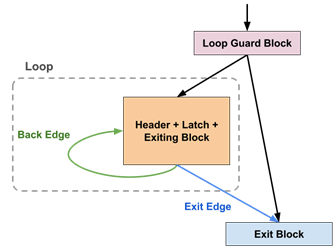
\includegraphics[width=0.9\textwidth]{content/3/chapter10/images/9.png}\\
Figure 10.9 – Structure and terminology of a rotated loop
\end{center}

To get a rotated loop, you can run LoopRotationPass over the original loop. To check if a loop is rotated, you can use the Loop::isRotatedForm method.

This rotated form is basically transforming an arbitrary loop into a do\{…\}while(…) loop (in C/C++) with some extra checks. More specifically, let's say we have the following for loop:

\begin{lstlisting}[style=styleCXX]
// `N` is not a constant
for (int i = 0; i < N; ++i){…}
\end{lstlisting}

Loop rotation effectively turns it into the following code:

\begin{lstlisting}[style=styleCXX]
if (i < N) {
	do {
		…
		++i;
	} while(i < N);
}
\end{lstlisting}

The highlighted boundary check in the preceding code is used to ensure that the loop won't execute if the i variable is out of bounds at the very beginning. We also call this check the loop guard, as shown in the preceding diagram.

In addition to the loop guard, we also found that a rotated loop has a combined header, latch, and exiting block. The rationale behind this is to ensure that every instruction in this block has the same execution count. This is a useful property for compiler optimizations such as loop vectorization.

With that, we have learned about the various loop terminologies and the definition of canonical loops in LLVM. In the next section, we will learn about some APIs that can help you inspect some of these properties and process loops in an efficient way

\subsubsubsection{10.4.2\hspace{0.2cm}Learning about loop infrastructure in LLVM}

In the Learning about loop representation in LLVM section, we learned about the high-level construction and important properties of a loop in LLVM IR. In this section, we are going to see what APIs are available for us to inspect those properties and further transform the loops. Let's start our discussion from the loop pass – the LLVM pass that applies to Loop instances.

In Chapter 9, Working with PassManager and AnalysisManager, we learned that there are different kinds of LLVM pass that work on different IR units – for instance, we have seen passes for Function and Module. These two kinds of passes have a similar function signature for their run method – the main entry point of an LLVM pass – as shown here:

\begin{lstlisting}[style=styleCXX]
PreservedAnalyses run(<IR unit class> &Unit,
					  <IR unit>AnalysisManager &AM);
\end{lstlisting}

Both of their run methods take two arguments – a reference to the IR unit instance and an AnalysisManager instance.

In contrast, a loop pass has a slightly more complicated run method signature, as
shown here:

\begin{lstlisting}[style=styleCXX]
PreservedAnalyses run(Loop &LP, LoopAnalysisManager &LAM,
					  LoopStandardAnalysisResults &LAR,
					  LPMUpdater &U);
\end{lstlisting}

The run method takes four arguments, but we already know about the first two. Here are the descriptions for the other two:

\begin{itemize}
\item The third argument, LoopStandardAnalysisResults, provides you with some analysis data instances, such as AAResults (alias analysis data), DominatorTree, and LoopInfo. These analyses are extensively used by many loop optimizations. However, most of them are managed by either FunctionAnalysisManager or ModuleAnalysisManager. This means that, originally, developers needed to implement more complicated methods – for example, using the OuterAnalysisManagerProxy class – to retrieve them. The LoopStandardAnalysisResults instance basically helps you retrieve this analysis data ahead of time.

\item The last argument is used for notifying PassManager of any newly added loops so that it can put those new loops into the queue before processing them later. It can also tell the PassManager to put the current loop into the queue again.

\end{itemize}

When we are writing a pass, we will want to use the analysis data provided by AnalysisManager – in this case, it is the LoopAnalysisManager instance. LoopAnalysisManager has a similar usage to other versions of AnalysisManager (FunctionAnalysisManager, for example) we learned about in the previous chapter. The only difference is that we need to supply an additional argument to the getResult method. Here is an example:

\begin{lstlisting}[style=styleCXX]
PreservedAnalyses run(Loop &LP, LoopAnalysisManager &LAM,
					  LoopStandardAnalysisResults &LAR,
					  LPMUpdater &U) {
	…
	LoopNest &LN = LAM.getResult<LoopNestAnalysis>(LP, LAR);
	…
}
\end{lstlisting}

LoopNest is the analysis data that's generated by LoopNestAnalysis. (We will talk about both shortly in the Dealing with nested loops section.)

As shown in the previous snippet, LoopAnalysisManager::getResult takes another LoopStandarAnalysisResults type argument, in addition to the Loop
instance.

Except for having different a run method signature and a slightly different usage of LoopAnalysisManager, developers can build their loop passes in the same way as other kinds of passes. Now that we've looked at the foundation provided by loop pass and AnalysisManager, it's time to look at some specialized loops. The first one we are going to introduce is the nested loop.

\hspace*{\fill} \\ %插入空行
\noindent
\textbf{Dealing with nested loops}

So far, we have been talking about loops with only one layer. However, nested loops – loops with other loop(s) enclosed in them – are also common in real-world scenarios. For example, most of the matrix multiplication implementations require at least two layers of loops.

Nested loops are usually depicted as a tree – called a loop tree. In a loop tree, every node represents a loop. If a node has a parent node, this means that the corresponding loop is enclosed within the loop being modeled by the parent. The following diagram shows an example of this:

\hspace*{\fill} \\ %插入空行
\begin{center}
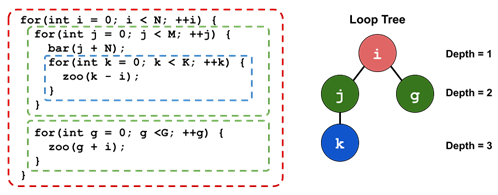
\includegraphics[width=0.9\textwidth]{content/3/chapter10/images/10.png}\\
Figure 10.10 – A loop tree example
\end{center}

In the preceding diagram, loops j and g are enclosed within loop i, so they are both child nodes of loop i in the loop tree. Similarly, loop k – the innermost loop – is modeled as the child node of loop j in the tree. 

The root of a loop tree also represents a top-level loop in a Function. Recall that, previously, we learned how to retrieve all Loop instances in a Function by iterating through the LoopInfo object – each of the Loop instances that were retrieved in this way are top-level loops. For a given Loop instance, we can retrieve its subloops at the next layer in a similar way. Here is an example:

\begin{lstlisting}[style=styleCXX]
// `LP` has the type of `Loop&`
for (Loop *SubLP : LP) {
	// `SubLP` is one of the sub-loops at the next layer
}
\end{lstlisting}

Note that the preceding snippet only traversed the subloops at the next level, rather than all the descendant subloops. To traverse all descendant subloops in a tree, you have two options:

\begin{itemize}
\item By using the Loop::getLoopsInPreorder() method, you can traverse all the descendant loops of a Loop instance in a pre-ordered fashion.

\item In the Iterating different IR units section, we have learned what GraphTraits is and how LLVM uses it for graph traversal. It turns out that LLVM also has a  default implementation of GraphTraits for the loop tree. Therefore, you can traverse a loop tree with existing graph iterators in LLVM, such as post-ordering and depth-first, to name a few. For example, the following code tries to traverse a loop tree rooted at RootL in a depth-first fashion:

\begin{lstlisting}[style=styleCXX]
#include "llvm/Analysis/LoopInfo.h"
#include "llvm/ADT/DepthFirstIterator.h"
…
// `RootL` has the type of `Loop*`
for (Loop *L : depth_first(RootL)) {
	// Work with `L`
}
\end{lstlisting}

With the help of GraphTraits, we can have more flexibility when it comes to traversing a loop tree.

\end{itemize}

In addition to dealing with individual loops in a loop tree, LLVM also provides a wrapper class that represents the whole structure – LoopNest. 

LoopNest is analysis data that's generated by LoopNestAnalysis. It encapsulates all the subloops in a given Loop instance and provides several "shortcut" APIs for commonly used functionalities. Here are some of the important ones:

\begin{itemize}
\item getOutermostLoop()/getInnermostLoop(): These utilities retrieve the outer/innermost Loop instances. These are pretty handy because many loop optimizations only apply to either the inner or outermost loop.

\item areAllLoopsSimplifyForm()/areAllLoopsRotatedForm(): These useful utilities tell you if all the enclosing loops are in a certain canonical form, as we mentioned in the previous section.

\item getPerfectLoops(…): You can use this to get all the perfect loops in the current loop hierarchy. By perfect loops, we are referring to loops that are nested together without a "gap" between them. Here is an example of perfect loops and non-perfect loops:

\begin{lstlisting}[style=styleCXX]
// Perfect loops
for(int i=…) {
	for(int j=…){…}
}
// Non-perfect loops
for(int x=…) {
	foo();
	for(int y=…){…}
}
\end{lstlisting}

In the non-perfect loops example, the foo call site is the gap between the upper and lower loops.

Perfect loops are preferrable in many loop optimizations. For example, it's easier to unroll perfectly nested loops – ideally, we only need to duplicate the body of the innermost loop.

\end{itemize}

With that, you've learned how to work with nested loops. In the next section, we are going to learn about another important topic for loop optimization: induction variables.

\hspace*{\fill} \\ %插入空行
\noindent
\textbf{Retrieving induction variables and their range}

The induction variable is a variable that progresses by a certain pattern in each loop iteration. It is the key to many loop optimizations. For example, in order to vectorize a loop, we need to know how the induction variable is used by the array – the data we want to put in a vector – within the loop. The induction variable can also help us resolve the trip count – the total number of iterations – of a loop. Before we dive into the details, the following diagram shows some terminology related to induction variables and where they're located in the loop:

\hspace*{\fill} \\ %插入空行
\begin{center}
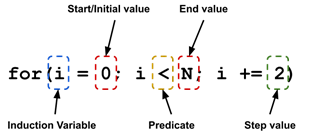
\includegraphics[width=0.9\textwidth]{content/3/chapter10/images/11.png}\\
Figure 10.11 – Terminology for an induction variable
\end{center}

Now, let's introduce some APIs that can help you retrieve the components shown in the preceding diagram.

First, let's talk about the induction variable. The Loop class already provides two convenient methods for retrieving the induction variable: getCanonicalInductionVariable and getInductionVariable. Both methods return a PHINode instance as the induction variable (if there are any). The first method can only be used if the induction variable starts from zero and only increments by one on each iteration. On the other hand, the second method can handle more complicated cases, but requires a ScalarEvolution instance as the argument.

ScalarEvolution is an interesting and powerful framework in LLVM. Simply put, it tries to track how values change – for example, through arithmetic operation – over the program path. Putting this into the context of loop optimization, it is used to capture recurrence value-changing behaviors in the loop, which has a strong relationship with the induction variable.

To find out more about the induction variable's behavior in a loop, you can retrieve an InductionDescriptor instance via Loop::getInductionDescriptor. An InductionDescriptor instance provides information such as the initial value, the step value, and the instruction that updates the induction variable at each iteration. The Loop class also provides another similar data structure for realizing the boundaries of the induction variable: the Loop::LoopBounds class. LoopBounds not only provides the initial and step values of the induction variable, but also the prospective ending value, as well as the predicate that's used for checking the exit condition. You can retrieve a LoopBounds instance via the Loop::getBounds method.

Loops are crucial for a program's runtime performance. In this section, we learned how loops are represented in LLVM IR and how to work with them. We also looked at their high-level concepts and various practical APIs for retrieving the desired loop properties. With this knowledge, you are one step closer to creating a more effective, aggressive loop optimization and gaining even higher performance from your target applications.













